
% Default to the notebook output style

    


% Inherit from the specified cell style.




    
\documentclass[11pt]{article}

    
    
    \usepackage[T1]{fontenc}
    % Nicer default font (+ math font) than Computer Modern for most use cases
    \usepackage{mathpazo}

    % Basic figure setup, for now with no caption control since it's done
    % automatically by Pandoc (which extracts ![](path) syntax from Markdown).
    \usepackage{graphicx}
    % We will generate all images so they have a width \maxwidth. This means
    % that they will get their normal width if they fit onto the page, but
    % are scaled down if they would overflow the margins.
    \makeatletter
    \def\maxwidth{\ifdim\Gin@nat@width>\linewidth\linewidth
    \else\Gin@nat@width\fi}
    \makeatother
    \let\Oldincludegraphics\includegraphics
    % Set max figure width to be 80% of text width, for now hardcoded.
    \renewcommand{\includegraphics}[1]{\Oldincludegraphics[width=.8\maxwidth]{#1}}
    % Ensure that by default, figures have no caption (until we provide a
    % proper Figure object with a Caption API and a way to capture that
    % in the conversion process - todo).
    \usepackage{caption}
    \DeclareCaptionLabelFormat{nolabel}{}
    \captionsetup{labelformat=nolabel}

    \usepackage{adjustbox} % Used to constrain images to a maximum size 
    \usepackage{xcolor} % Allow colors to be defined
    \usepackage{enumerate} % Needed for markdown enumerations to work
    \usepackage{geometry} % Used to adjust the document margins
    \usepackage{amsmath} % Equations
    \usepackage{amssymb} % Equations
    \usepackage{textcomp} % defines textquotesingle
    % Hack from http://tex.stackexchange.com/a/47451/13684:
    \AtBeginDocument{%
        \def\PYZsq{\textquotesingle}% Upright quotes in Pygmentized code
    }
    \usepackage{upquote} % Upright quotes for verbatim code
    \usepackage{eurosym} % defines \euro
    \usepackage[mathletters]{ucs} % Extended unicode (utf-8) support
    \usepackage[utf8x]{inputenc} % Allow utf-8 characters in the tex document
    \usepackage{fancyvrb} % verbatim replacement that allows latex
    \usepackage{grffile} % extends the file name processing of package graphics 
                         % to support a larger range 
    % The hyperref package gives us a pdf with properly built
    % internal navigation ('pdf bookmarks' for the table of contents,
    % internal cross-reference links, web links for URLs, etc.)
    \usepackage{hyperref}
    \usepackage{longtable} % longtable support required by pandoc >1.10
    \usepackage{booktabs}  % table support for pandoc > 1.12.2
    \usepackage[inline]{enumitem} % IRkernel/repr support (it uses the enumerate* environment)
    \usepackage[normalem]{ulem} % ulem is needed to support strikethroughs (\sout)
                                % normalem makes italics be italics, not underlines
    

    
    
    % Colors for the hyperref package
    \definecolor{urlcolor}{rgb}{0,.145,.698}
    \definecolor{linkcolor}{rgb}{.71,0.21,0.01}
    \definecolor{citecolor}{rgb}{.12,.54,.11}

    % ANSI colors
    \definecolor{ansi-black}{HTML}{3E424D}
    \definecolor{ansi-black-intense}{HTML}{282C36}
    \definecolor{ansi-red}{HTML}{E75C58}
    \definecolor{ansi-red-intense}{HTML}{B22B31}
    \definecolor{ansi-green}{HTML}{00A250}
    \definecolor{ansi-green-intense}{HTML}{007427}
    \definecolor{ansi-yellow}{HTML}{DDB62B}
    \definecolor{ansi-yellow-intense}{HTML}{B27D12}
    \definecolor{ansi-blue}{HTML}{208FFB}
    \definecolor{ansi-blue-intense}{HTML}{0065CA}
    \definecolor{ansi-magenta}{HTML}{D160C4}
    \definecolor{ansi-magenta-intense}{HTML}{A03196}
    \definecolor{ansi-cyan}{HTML}{60C6C8}
    \definecolor{ansi-cyan-intense}{HTML}{258F8F}
    \definecolor{ansi-white}{HTML}{C5C1B4}
    \definecolor{ansi-white-intense}{HTML}{A1A6B2}

    % commands and environments needed by pandoc snippets
    % extracted from the output of `pandoc -s`
    \providecommand{\tightlist}{%
      \setlength{\itemsep}{0pt}\setlength{\parskip}{0pt}}
    \DefineVerbatimEnvironment{Highlighting}{Verbatim}{commandchars=\\\{\}}
    % Add ',fontsize=\small' for more characters per line
    \newenvironment{Shaded}{}{}
    \newcommand{\KeywordTok}[1]{\textcolor[rgb]{0.00,0.44,0.13}{\textbf{{#1}}}}
    \newcommand{\DataTypeTok}[1]{\textcolor[rgb]{0.56,0.13,0.00}{{#1}}}
    \newcommand{\DecValTok}[1]{\textcolor[rgb]{0.25,0.63,0.44}{{#1}}}
    \newcommand{\BaseNTok}[1]{\textcolor[rgb]{0.25,0.63,0.44}{{#1}}}
    \newcommand{\FloatTok}[1]{\textcolor[rgb]{0.25,0.63,0.44}{{#1}}}
    \newcommand{\CharTok}[1]{\textcolor[rgb]{0.25,0.44,0.63}{{#1}}}
    \newcommand{\StringTok}[1]{\textcolor[rgb]{0.25,0.44,0.63}{{#1}}}
    \newcommand{\CommentTok}[1]{\textcolor[rgb]{0.38,0.63,0.69}{\textit{{#1}}}}
    \newcommand{\OtherTok}[1]{\textcolor[rgb]{0.00,0.44,0.13}{{#1}}}
    \newcommand{\AlertTok}[1]{\textcolor[rgb]{1.00,0.00,0.00}{\textbf{{#1}}}}
    \newcommand{\FunctionTok}[1]{\textcolor[rgb]{0.02,0.16,0.49}{{#1}}}
    \newcommand{\RegionMarkerTok}[1]{{#1}}
    \newcommand{\ErrorTok}[1]{\textcolor[rgb]{1.00,0.00,0.00}{\textbf{{#1}}}}
    \newcommand{\NormalTok}[1]{{#1}}
    
    % Additional commands for more recent versions of Pandoc
    \newcommand{\ConstantTok}[1]{\textcolor[rgb]{0.53,0.00,0.00}{{#1}}}
    \newcommand{\SpecialCharTok}[1]{\textcolor[rgb]{0.25,0.44,0.63}{{#1}}}
    \newcommand{\VerbatimStringTok}[1]{\textcolor[rgb]{0.25,0.44,0.63}{{#1}}}
    \newcommand{\SpecialStringTok}[1]{\textcolor[rgb]{0.73,0.40,0.53}{{#1}}}
    \newcommand{\ImportTok}[1]{{#1}}
    \newcommand{\DocumentationTok}[1]{\textcolor[rgb]{0.73,0.13,0.13}{\textit{{#1}}}}
    \newcommand{\AnnotationTok}[1]{\textcolor[rgb]{0.38,0.63,0.69}{\textbf{\textit{{#1}}}}}
    \newcommand{\CommentVarTok}[1]{\textcolor[rgb]{0.38,0.63,0.69}{\textbf{\textit{{#1}}}}}
    \newcommand{\VariableTok}[1]{\textcolor[rgb]{0.10,0.09,0.49}{{#1}}}
    \newcommand{\ControlFlowTok}[1]{\textcolor[rgb]{0.00,0.44,0.13}{\textbf{{#1}}}}
    \newcommand{\OperatorTok}[1]{\textcolor[rgb]{0.40,0.40,0.40}{{#1}}}
    \newcommand{\BuiltInTok}[1]{{#1}}
    \newcommand{\ExtensionTok}[1]{{#1}}
    \newcommand{\PreprocessorTok}[1]{\textcolor[rgb]{0.74,0.48,0.00}{{#1}}}
    \newcommand{\AttributeTok}[1]{\textcolor[rgb]{0.49,0.56,0.16}{{#1}}}
    \newcommand{\InformationTok}[1]{\textcolor[rgb]{0.38,0.63,0.69}{\textbf{\textit{{#1}}}}}
    \newcommand{\WarningTok}[1]{\textcolor[rgb]{0.38,0.63,0.69}{\textbf{\textit{{#1}}}}}
    
    
    % Define a nice break command that doesn't care if a line doesn't already
    % exist.
    \def\br{\hspace*{\fill} \\* }
    % Math Jax compatability definitions
    \def\gt{>}
    \def\lt{<}
    % Document parameters
    \title{lecture\_10}
    
    
    

    % Pygments definitions
    
\makeatletter
\def\PY@reset{\let\PY@it=\relax \let\PY@bf=\relax%
    \let\PY@ul=\relax \let\PY@tc=\relax%
    \let\PY@bc=\relax \let\PY@ff=\relax}
\def\PY@tok#1{\csname PY@tok@#1\endcsname}
\def\PY@toks#1+{\ifx\relax#1\empty\else%
    \PY@tok{#1}\expandafter\PY@toks\fi}
\def\PY@do#1{\PY@bc{\PY@tc{\PY@ul{%
    \PY@it{\PY@bf{\PY@ff{#1}}}}}}}
\def\PY#1#2{\PY@reset\PY@toks#1+\relax+\PY@do{#2}}

\expandafter\def\csname PY@tok@gd\endcsname{\def\PY@tc##1{\textcolor[rgb]{0.63,0.00,0.00}{##1}}}
\expandafter\def\csname PY@tok@gu\endcsname{\let\PY@bf=\textbf\def\PY@tc##1{\textcolor[rgb]{0.50,0.00,0.50}{##1}}}
\expandafter\def\csname PY@tok@gt\endcsname{\def\PY@tc##1{\textcolor[rgb]{0.00,0.27,0.87}{##1}}}
\expandafter\def\csname PY@tok@gs\endcsname{\let\PY@bf=\textbf}
\expandafter\def\csname PY@tok@gr\endcsname{\def\PY@tc##1{\textcolor[rgb]{1.00,0.00,0.00}{##1}}}
\expandafter\def\csname PY@tok@cm\endcsname{\let\PY@it=\textit\def\PY@tc##1{\textcolor[rgb]{0.25,0.50,0.50}{##1}}}
\expandafter\def\csname PY@tok@vg\endcsname{\def\PY@tc##1{\textcolor[rgb]{0.10,0.09,0.49}{##1}}}
\expandafter\def\csname PY@tok@vi\endcsname{\def\PY@tc##1{\textcolor[rgb]{0.10,0.09,0.49}{##1}}}
\expandafter\def\csname PY@tok@mh\endcsname{\def\PY@tc##1{\textcolor[rgb]{0.40,0.40,0.40}{##1}}}
\expandafter\def\csname PY@tok@cs\endcsname{\let\PY@it=\textit\def\PY@tc##1{\textcolor[rgb]{0.25,0.50,0.50}{##1}}}
\expandafter\def\csname PY@tok@ge\endcsname{\let\PY@it=\textit}
\expandafter\def\csname PY@tok@vc\endcsname{\def\PY@tc##1{\textcolor[rgb]{0.10,0.09,0.49}{##1}}}
\expandafter\def\csname PY@tok@il\endcsname{\def\PY@tc##1{\textcolor[rgb]{0.40,0.40,0.40}{##1}}}
\expandafter\def\csname PY@tok@go\endcsname{\def\PY@tc##1{\textcolor[rgb]{0.53,0.53,0.53}{##1}}}
\expandafter\def\csname PY@tok@cp\endcsname{\def\PY@tc##1{\textcolor[rgb]{0.74,0.48,0.00}{##1}}}
\expandafter\def\csname PY@tok@gi\endcsname{\def\PY@tc##1{\textcolor[rgb]{0.00,0.63,0.00}{##1}}}
\expandafter\def\csname PY@tok@gh\endcsname{\let\PY@bf=\textbf\def\PY@tc##1{\textcolor[rgb]{0.00,0.00,0.50}{##1}}}
\expandafter\def\csname PY@tok@ni\endcsname{\let\PY@bf=\textbf\def\PY@tc##1{\textcolor[rgb]{0.60,0.60,0.60}{##1}}}
\expandafter\def\csname PY@tok@nl\endcsname{\def\PY@tc##1{\textcolor[rgb]{0.63,0.63,0.00}{##1}}}
\expandafter\def\csname PY@tok@nn\endcsname{\let\PY@bf=\textbf\def\PY@tc##1{\textcolor[rgb]{0.00,0.00,1.00}{##1}}}
\expandafter\def\csname PY@tok@no\endcsname{\def\PY@tc##1{\textcolor[rgb]{0.53,0.00,0.00}{##1}}}
\expandafter\def\csname PY@tok@na\endcsname{\def\PY@tc##1{\textcolor[rgb]{0.49,0.56,0.16}{##1}}}
\expandafter\def\csname PY@tok@nb\endcsname{\def\PY@tc##1{\textcolor[rgb]{0.00,0.50,0.00}{##1}}}
\expandafter\def\csname PY@tok@nc\endcsname{\let\PY@bf=\textbf\def\PY@tc##1{\textcolor[rgb]{0.00,0.00,1.00}{##1}}}
\expandafter\def\csname PY@tok@nd\endcsname{\def\PY@tc##1{\textcolor[rgb]{0.67,0.13,1.00}{##1}}}
\expandafter\def\csname PY@tok@ne\endcsname{\let\PY@bf=\textbf\def\PY@tc##1{\textcolor[rgb]{0.82,0.25,0.23}{##1}}}
\expandafter\def\csname PY@tok@nf\endcsname{\def\PY@tc##1{\textcolor[rgb]{0.00,0.00,1.00}{##1}}}
\expandafter\def\csname PY@tok@si\endcsname{\let\PY@bf=\textbf\def\PY@tc##1{\textcolor[rgb]{0.73,0.40,0.53}{##1}}}
\expandafter\def\csname PY@tok@s2\endcsname{\def\PY@tc##1{\textcolor[rgb]{0.73,0.13,0.13}{##1}}}
\expandafter\def\csname PY@tok@nt\endcsname{\let\PY@bf=\textbf\def\PY@tc##1{\textcolor[rgb]{0.00,0.50,0.00}{##1}}}
\expandafter\def\csname PY@tok@nv\endcsname{\def\PY@tc##1{\textcolor[rgb]{0.10,0.09,0.49}{##1}}}
\expandafter\def\csname PY@tok@s1\endcsname{\def\PY@tc##1{\textcolor[rgb]{0.73,0.13,0.13}{##1}}}
\expandafter\def\csname PY@tok@ch\endcsname{\let\PY@it=\textit\def\PY@tc##1{\textcolor[rgb]{0.25,0.50,0.50}{##1}}}
\expandafter\def\csname PY@tok@m\endcsname{\def\PY@tc##1{\textcolor[rgb]{0.40,0.40,0.40}{##1}}}
\expandafter\def\csname PY@tok@gp\endcsname{\let\PY@bf=\textbf\def\PY@tc##1{\textcolor[rgb]{0.00,0.00,0.50}{##1}}}
\expandafter\def\csname PY@tok@sh\endcsname{\def\PY@tc##1{\textcolor[rgb]{0.73,0.13,0.13}{##1}}}
\expandafter\def\csname PY@tok@ow\endcsname{\let\PY@bf=\textbf\def\PY@tc##1{\textcolor[rgb]{0.67,0.13,1.00}{##1}}}
\expandafter\def\csname PY@tok@sx\endcsname{\def\PY@tc##1{\textcolor[rgb]{0.00,0.50,0.00}{##1}}}
\expandafter\def\csname PY@tok@bp\endcsname{\def\PY@tc##1{\textcolor[rgb]{0.00,0.50,0.00}{##1}}}
\expandafter\def\csname PY@tok@c1\endcsname{\let\PY@it=\textit\def\PY@tc##1{\textcolor[rgb]{0.25,0.50,0.50}{##1}}}
\expandafter\def\csname PY@tok@o\endcsname{\def\PY@tc##1{\textcolor[rgb]{0.40,0.40,0.40}{##1}}}
\expandafter\def\csname PY@tok@kc\endcsname{\let\PY@bf=\textbf\def\PY@tc##1{\textcolor[rgb]{0.00,0.50,0.00}{##1}}}
\expandafter\def\csname PY@tok@c\endcsname{\let\PY@it=\textit\def\PY@tc##1{\textcolor[rgb]{0.25,0.50,0.50}{##1}}}
\expandafter\def\csname PY@tok@mf\endcsname{\def\PY@tc##1{\textcolor[rgb]{0.40,0.40,0.40}{##1}}}
\expandafter\def\csname PY@tok@err\endcsname{\def\PY@bc##1{\setlength{\fboxsep}{0pt}\fcolorbox[rgb]{1.00,0.00,0.00}{1,1,1}{\strut ##1}}}
\expandafter\def\csname PY@tok@mb\endcsname{\def\PY@tc##1{\textcolor[rgb]{0.40,0.40,0.40}{##1}}}
\expandafter\def\csname PY@tok@ss\endcsname{\def\PY@tc##1{\textcolor[rgb]{0.10,0.09,0.49}{##1}}}
\expandafter\def\csname PY@tok@sr\endcsname{\def\PY@tc##1{\textcolor[rgb]{0.73,0.40,0.53}{##1}}}
\expandafter\def\csname PY@tok@mo\endcsname{\def\PY@tc##1{\textcolor[rgb]{0.40,0.40,0.40}{##1}}}
\expandafter\def\csname PY@tok@kd\endcsname{\let\PY@bf=\textbf\def\PY@tc##1{\textcolor[rgb]{0.00,0.50,0.00}{##1}}}
\expandafter\def\csname PY@tok@mi\endcsname{\def\PY@tc##1{\textcolor[rgb]{0.40,0.40,0.40}{##1}}}
\expandafter\def\csname PY@tok@kn\endcsname{\let\PY@bf=\textbf\def\PY@tc##1{\textcolor[rgb]{0.00,0.50,0.00}{##1}}}
\expandafter\def\csname PY@tok@cpf\endcsname{\let\PY@it=\textit\def\PY@tc##1{\textcolor[rgb]{0.25,0.50,0.50}{##1}}}
\expandafter\def\csname PY@tok@kr\endcsname{\let\PY@bf=\textbf\def\PY@tc##1{\textcolor[rgb]{0.00,0.50,0.00}{##1}}}
\expandafter\def\csname PY@tok@s\endcsname{\def\PY@tc##1{\textcolor[rgb]{0.73,0.13,0.13}{##1}}}
\expandafter\def\csname PY@tok@kp\endcsname{\def\PY@tc##1{\textcolor[rgb]{0.00,0.50,0.00}{##1}}}
\expandafter\def\csname PY@tok@w\endcsname{\def\PY@tc##1{\textcolor[rgb]{0.73,0.73,0.73}{##1}}}
\expandafter\def\csname PY@tok@kt\endcsname{\def\PY@tc##1{\textcolor[rgb]{0.69,0.00,0.25}{##1}}}
\expandafter\def\csname PY@tok@sc\endcsname{\def\PY@tc##1{\textcolor[rgb]{0.73,0.13,0.13}{##1}}}
\expandafter\def\csname PY@tok@sb\endcsname{\def\PY@tc##1{\textcolor[rgb]{0.73,0.13,0.13}{##1}}}
\expandafter\def\csname PY@tok@k\endcsname{\let\PY@bf=\textbf\def\PY@tc##1{\textcolor[rgb]{0.00,0.50,0.00}{##1}}}
\expandafter\def\csname PY@tok@se\endcsname{\let\PY@bf=\textbf\def\PY@tc##1{\textcolor[rgb]{0.73,0.40,0.13}{##1}}}
\expandafter\def\csname PY@tok@sd\endcsname{\let\PY@it=\textit\def\PY@tc##1{\textcolor[rgb]{0.73,0.13,0.13}{##1}}}

\def\PYZbs{\char`\\}
\def\PYZus{\char`\_}
\def\PYZob{\char`\{}
\def\PYZcb{\char`\}}
\def\PYZca{\char`\^}
\def\PYZam{\char`\&}
\def\PYZlt{\char`\<}
\def\PYZgt{\char`\>}
\def\PYZsh{\char`\#}
\def\PYZpc{\char`\%}
\def\PYZdl{\char`\$}
\def\PYZhy{\char`\-}
\def\PYZsq{\char`\'}
\def\PYZdq{\char`\"}
\def\PYZti{\char`\~}
% for compatibility with earlier versions
\def\PYZat{@}
\def\PYZlb{[}
\def\PYZrb{]}
\makeatother


    % Exact colors from NB
    \definecolor{incolor}{rgb}{0.0, 0.0, 0.5}
    \definecolor{outcolor}{rgb}{0.545, 0.0, 0.0}



    
    % Prevent overflowing lines due to hard-to-break entities
    \sloppy 
    % Setup hyperref package
    \hypersetup{
      breaklinks=true,  % so long urls are correctly broken across lines
      colorlinks=true,
      urlcolor=urlcolor,
      linkcolor=linkcolor,
      citecolor=citecolor,
      }
    % Slightly bigger margins than the latex defaults
    
    \geometry{verbose,tmargin=1in,bmargin=1in,lmargin=1in,rmargin=1in}
    
    

    \begin{document}
    
    
    \maketitle
    
    

    
    \begin{Verbatim}[commandchars=\\\{\}]
{\color{incolor}In [{\color{incolor}14}]:} \PY{c}{\PYZpc{}plot \PYZhy{}\PYZhy{}format svg}
\end{Verbatim}

    \begin{Verbatim}[commandchars=\\\{\}]
{\color{incolor}In [{\color{incolor}15}]:} \PY{n}{setdefaults}
\end{Verbatim}

    \section{Gauss Elimination}\label{gauss-elimination}

\subsubsection{Solving sets of equations with matrix
operations}\label{solving-sets-of-equations-with-matrix-operations}

The number of dimensions of a matrix indicate the degrees of freedom of
the system you are solving.

If you have a set of known output, \(y_{1},~y_{2},~...y_{N}\) and a set
of equations that relate unknown inputs, \(x_{1},~x_{2},~...x_{N}\),
then these can be written in a vector matrix format as:

\(y=Ax\)

Consider a problem with 2 DOF:

\(x_{1}+3x_{2}=1\)

\(2x_{1}+x_{2}=1\)

\(\left[ \begin{array}{cc} 1 & 3 \\ 2 & 1 \end{array} \right] \left[\begin{array}{c} x_{1} \\ x_{2} \end{array}\right]= \left[\begin{array}{c} 1 \\ 1\end{array}\right]\)

The solution for \(x_{1}\) and \(x_{2}\) is the intersection of two
lines:

    \begin{Verbatim}[commandchars=\\\{\}]
{\color{incolor}In [{\color{incolor}16}]:} \PY{n}{x21}\PY{p}{=}\PY{p}{[}\PY{o}{\PYZhy{}}\PY{l+m+mi}{2}\PY{p}{:}\PY{l+m+mi}{2}\PY{p}{]}\PY{p}{;}
         \PY{n}{x11}\PY{p}{=}\PY{l+m+mi}{1}\PY{o}{\PYZhy{}}\PY{l+m+mi}{3}\PY{o}{*}\PY{n}{x21}\PY{p}{;}
         \PY{n}{x21}\PY{p}{=}\PY{p}{[}\PY{o}{\PYZhy{}}\PY{l+m+mi}{2}\PY{p}{:}\PY{l+m+mi}{2}\PY{p}{]}\PY{p}{;}
         \PY{n}{x22}\PY{p}{=}\PY{l+m+mi}{1}\PY{o}{\PYZhy{}}\PY{l+m+mi}{2}\PY{o}{*}\PY{n}{x21}\PY{p}{;}
         \PY{n+nb}{plot}\PY{p}{(}\PY{n}{x11}\PY{p}{,}\PY{n}{x21}\PY{p}{,}\PY{n}{x21}\PY{p}{,}\PY{n}{x22}\PY{p}{)}
\end{Verbatim}

    \begin{center}
    \adjustimage{max size={0.9\linewidth}{0.9\paperheight}}{lecture_10_files/lecture_10_3_0.pdf}
    \end{center}
    { \hspace*{\fill} \\}
    
    For a $3\times3$ matrix, the solution is the intersection of the 3
planes.

\(10x_{1}+2x_{2}+x_{3}=1\)

\(2x_{1}+x_{2}+x_{3}=1\)

\(x_{1}+2x_{2}+10x_{3}=1\)

$\left[ \begin{array}{ccc} 10 & 2 & 1 \\ 2 & 1 & 1 \\ 1 & 2 & 10\end{array} \right]
  \left[\begin{array}{c} x_{1} \\ x_{2} \\ x_{3} \end{array}\right]=
    \left[\begin{array}{c} 1 \\ 1 \\ 1\end{array}\right]$

    \begin{Verbatim}[commandchars=\\\{\}]
{\color{incolor}In [{\color{incolor}17}]:} \PY{n}{x11}\PY{p}{=}\PY{n+nb}{linspace}\PY{p}{(}\PY{o}{\PYZhy{}}\PY{l+m+mi}{2}\PY{p}{,}\PY{l+m+mi}{2}\PY{p}{,}\PY{l+m+mi}{5}\PY{p}{)}\PY{p}{;}
         \PY{n}{x12}\PY{p}{=}\PY{n+nb}{linspace}\PY{p}{(}\PY{o}{\PYZhy{}}\PY{l+m+mi}{2}\PY{p}{,}\PY{l+m+mi}{2}\PY{p}{,}\PY{l+m+mi}{5}\PY{p}{)}\PY{p}{;}
         \PY{p}{[}\PY{n}{X11}\PY{p}{,}\PY{n}{X12}\PY{p}{]}\PY{p}{=}\PY{n+nb}{meshgrid}\PY{p}{(}\PY{n}{x11}\PY{p}{,}\PY{n}{x12}\PY{p}{)}\PY{p}{;}
         \PY{n}{X13}\PY{p}{=}\PY{l+m+mi}{1}\PY{o}{\PYZhy{}}\PY{l+m+mi}{10}\PY{o}{*}\PY{n}{X11}\PY{o}{\PYZhy{}}\PY{l+m+mi}{2}\PY{o}{*}\PY{n}{X22}\PY{p}{;}
         
         \PY{n}{x21}\PY{p}{=}\PY{n+nb}{linspace}\PY{p}{(}\PY{o}{\PYZhy{}}\PY{l+m+mi}{2}\PY{p}{,}\PY{l+m+mi}{2}\PY{p}{,}\PY{l+m+mi}{5}\PY{p}{)}\PY{p}{;}
         \PY{n}{x22}\PY{p}{=}\PY{n+nb}{linspace}\PY{p}{(}\PY{o}{\PYZhy{}}\PY{l+m+mi}{2}\PY{p}{,}\PY{l+m+mi}{2}\PY{p}{,}\PY{l+m+mi}{5}\PY{p}{)}\PY{p}{;}
         \PY{p}{[}\PY{n}{X21}\PY{p}{,}\PY{n}{X22}\PY{p}{]}\PY{p}{=}\PY{n+nb}{meshgrid}\PY{p}{(}\PY{n}{x21}\PY{p}{,}\PY{n}{x22}\PY{p}{)}\PY{p}{;}
         \PY{n}{X23}\PY{p}{=}\PY{l+m+mi}{1}\PY{o}{\PYZhy{}}\PY{l+m+mi}{2}\PY{o}{*}\PY{n}{X11}\PY{o}{\PYZhy{}}\PY{n}{X22}\PY{p}{;}
         
         \PY{n}{x31}\PY{p}{=}\PY{n+nb}{linspace}\PY{p}{(}\PY{o}{\PYZhy{}}\PY{l+m+mi}{2}\PY{p}{,}\PY{l+m+mi}{2}\PY{p}{,}\PY{l+m+mi}{5}\PY{p}{)}\PY{p}{;}
         \PY{n}{x32}\PY{p}{=}\PY{n+nb}{linspace}\PY{p}{(}\PY{o}{\PYZhy{}}\PY{l+m+mi}{2}\PY{p}{,}\PY{l+m+mi}{2}\PY{p}{,}\PY{l+m+mi}{5}\PY{p}{)}\PY{p}{;}
         \PY{p}{[}\PY{n}{X31}\PY{p}{,}\PY{n}{X32}\PY{p}{]}\PY{p}{=}\PY{n+nb}{meshgrid}\PY{p}{(}\PY{n}{x31}\PY{p}{,}\PY{n}{x32}\PY{p}{)}\PY{p}{;}
         \PY{n}{X33}\PY{p}{=}\PY{l+m+mi}{1}\PY{o}{/}\PY{l+m+mi}{10}\PY{o}{*}\PY{p}{(}\PY{l+m+mi}{1}\PY{o}{\PYZhy{}}\PY{n}{X31}\PY{o}{\PYZhy{}}\PY{l+m+mi}{2}\PY{o}{*}\PY{n}{X32}\PY{p}{)}\PY{p}{;}
         
         \PY{n+nb}{mesh}\PY{p}{(}\PY{n}{X11}\PY{p}{,}\PY{n}{X12}\PY{p}{,}\PY{n}{X13}\PY{p}{)}\PY{p}{;}
         \PY{n+nb}{hold} \PY{n}{on}\PY{p}{;}
         \PY{n+nb}{mesh}\PY{p}{(}\PY{n}{X21}\PY{p}{,}\PY{n}{X22}\PY{p}{,}\PY{n}{X23}\PY{p}{)}
         \PY{n+nb}{mesh}\PY{p}{(}\PY{n}{X31}\PY{p}{,}\PY{n}{X32}\PY{p}{,}\PY{n}{X33}\PY{p}{)}
         \PY{n}{x}\PY{p}{=}\PY{p}{[}\PY{l+m+mi}{10}\PY{p}{,}\PY{l+m+mi}{2}\PY{p}{,} \PY{l+m+mi}{1}\PY{p}{;}\PY{l+m+mi}{2}\PY{p}{,}\PY{l+m+mi}{1}\PY{p}{,} \PY{l+m+mi}{1}\PY{p}{;} \PY{l+m+mi}{1}\PY{p}{,} \PY{l+m+mi}{2}\PY{p}{,} \PY{l+m+mi}{10}\PY{p}{]}\PY{o}{\PYZbs{}}\PY{p}{[}\PY{l+m+mi}{1}\PY{p}{;}\PY{l+m+mi}{1}\PY{p}{;}\PY{l+m+mi}{1}\PY{p}{]}\PY{p}{;}
         \PY{n}{plot3}\PY{p}{(}\PY{n}{x}\PY{p}{(}\PY{l+m+mi}{1}\PY{p}{)}\PY{p}{,}\PY{n}{x}\PY{p}{(}\PY{l+m+mi}{2}\PY{p}{)}\PY{p}{,}\PY{n}{x}\PY{p}{(}\PY{l+m+mi}{3}\PY{p}{)}\PY{p}{,}\PY{l+s}{\PYZsq{}}\PY{l+s}{o\PYZsq{}}\PY{p}{)}
         \PY{n+nb}{view}\PY{p}{(}\PY{l+m+mi}{45}\PY{p}{,}\PY{l+m+mi}{45}\PY{p}{)}
\end{Verbatim}

    \begin{Verbatim}[commandchars=\\\{\}]
error: 'X22' undefined near line 1 column 16
error: 'X13' undefined near line 1 column 14
error: evaluating argument list element number 3

    \end{Verbatim}

    \begin{center}
    \adjustimage{max size={0.9\linewidth}{0.9\paperheight}}{lecture_10_files/lecture_10_5_1.pdf}
    \end{center}
    { \hspace*{\fill} \\}
    
    After 3 DOF problems, the solutions are described as \emph{hyperplane}
intersections. Which are even harder to visualize

    \subsection{Gauss elimination}\label{gauss-elimination}

\subsubsection{Solving sets of equations
systematically}\label{solving-sets-of-equations-systematically}

$\left[
\begin{array}{ccc|c}
   & A & & y \\
10 & 2 & 1 & 1\\
2 & 1 & 1  & 1 \\
1 & 2 & 10 & 1\end{array}
\right] $

Ay(2,:)-Ay(1,:)/5 = ({[}2 1 1 1{]}-1/5{[}10 2 1 1{]})

$\left[
\begin{array}{ccc|c}
   & A & & y \\
10 & 2 & 1 & 1\\
0 & 3/5 & 4/5  & 4/5 \\
1 & 2 & 10 & 1\end{array}
\right] $

Ay(3,:)-Ay(1,:)/10 = ({[}1 2 10 1{]}-1/10{[}10 2 1 1{]})

$\left[
\begin{array}{ccc|c}
   & A & & y \\
10 & 2 & 1 & 1\\
0 & 3/5 & 4/5  & 4/5 \\
0 & 1.8 & 9.9 & 0.9\end{array}
\right] $

Ay(3,:)-1.8*5/3*Ay(2,:) = ({[}0 1.8 9.9 0.9{]}-3*{[}0 3/5 4/5 4/5{]})

$\left[
\begin{array}{ccc|c}
   & A & & y \\
10 & 2 & 1 & 1\\
0 & 3/5 & 4/5  & 4/5 \\
0 & 0 & 7.5 & -1.5\end{array}
\right] $

now, \(7.5x_{3}=-1.5\) so \(x_{3}=-\frac{1}{5}\)

then, \(3/5x_{2}+4/5(-1/5)=1\) so \(x_{2}=\frac{8}{5}\)

finally, \$10x\_\{1\}+2(8/5)

    Consider the problem again from the intro to Linear Algebra, 4 masses
are connected in series to 4 springs with K=10 N/m. What are the final
positions of the masses?

\begin{figure}[htbp]
\centering
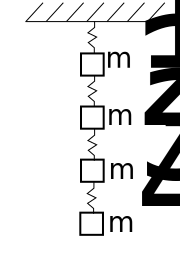
\includegraphics{../lecture_09/mass_springs.svg}
\caption{Springs-masses}
\end{figure}

The masses haves the following amounts, 1, 2, 3, and 4 kg for masses
1-4. Using a FBD for each mass:

\(m_{1}g+k(x_{2}-x_{1})-kx_{1}=0\)

\(m_{2}g+k(x_{3}-x_{2})-k(x_{2}-x_{1})=0\)

\(m_{3}g+k(x_{4}-x_{3})-k(x_{3}-x_{2})=0\)

\(m_{4}g-k(x_{4}-x_{3})=0\)

in matrix form:

\(\left[ \begin{array}{cccc} 2k & -k & 0 & 0 \\ -k & 2k & -k & 0 \\ 0 & -k & 2k & -k \\ 0 & 0 & -k & k \end{array} \right] \left[ \begin{array}{c} x_{1} \\ x_{2} \\ x_{3} \\ x_{4} \end{array} \right]= \left[ \begin{array}{c} m_{1}g \\ m_{2}g \\ m_{3}g \\ m_{4}g \end{array} \right]\)

    \begin{Verbatim}[commandchars=\\\{\}]
{\color{incolor}In [{\color{incolor}18}]:} \PY{n}{k}\PY{p}{=}\PY{l+m+mi}{10}\PY{p}{;} \PY{c}{\PYZpc{} N/m}
         \PY{n}{m1}\PY{p}{=}\PY{l+m+mi}{1}\PY{p}{;} \PY{c}{\PYZpc{} kg}
         \PY{n}{m2}\PY{p}{=}\PY{l+m+mi}{2}\PY{p}{;}
         \PY{n}{m3}\PY{p}{=}\PY{l+m+mi}{3}\PY{p}{;}
         \PY{n}{m4}\PY{p}{=}\PY{l+m+mi}{4}\PY{p}{;}
         \PY{n}{g}\PY{p}{=}\PY{l+m+mf}{9.81}\PY{p}{;} \PY{c}{\PYZpc{} m/s\PYZca{}2}
         \PY{n}{K}\PY{p}{=}\PY{p}{[}\PY{l+m+mi}{2}\PY{o}{*}\PY{n}{k} \PY{o}{\PYZhy{}}\PY{n}{k} \PY{l+m+mi}{0} \PY{l+m+mi}{0}\PY{p}{;} \PY{o}{\PYZhy{}}\PY{n}{k} \PY{l+m+mi}{2}\PY{o}{*}\PY{n}{k} \PY{o}{\PYZhy{}}\PY{n}{k} \PY{l+m+mi}{0}\PY{p}{;} \PY{l+m+mi}{0} \PY{o}{\PYZhy{}}\PY{n}{k} \PY{l+m+mi}{2}\PY{o}{*}\PY{n}{k} \PY{o}{\PYZhy{}}\PY{n}{k}\PY{p}{;} \PY{l+m+mi}{0} \PY{l+m+mi}{0} \PY{o}{\PYZhy{}}\PY{n}{k} \PY{n}{k}\PY{p}{]}
         \PY{n}{y}\PY{p}{=}\PY{p}{[}\PY{n}{m1}\PY{o}{*}\PY{n}{g}\PY{p}{;}\PY{n}{m2}\PY{o}{*}\PY{n}{g}\PY{p}{;}\PY{n}{m3}\PY{o}{*}\PY{n}{g}\PY{p}{;}\PY{n}{m4}\PY{o}{*}\PY{n}{g}\PY{p}{]}
\end{Verbatim}

    \begin{Verbatim}[commandchars=\\\{\}]
K =

   20  -10    0    0
  -10   20  -10    0
    0  -10   20  -10
    0    0  -10   10

y =

    9.8100
   19.6200
   29.4300
   39.2400


    \end{Verbatim}

    \begin{Verbatim}[commandchars=\\\{\}]
{\color{incolor}In [{\color{incolor}19}]:} \PY{n}{K1}\PY{p}{=}\PY{p}{[}\PY{n}{K} \PY{n}{y}\PY{p}{]}\PY{p}{;}
         \PY{n}{K1}\PY{p}{(}\PY{l+m+mi}{2}\PY{p}{,}\PY{p}{:}\PY{p}{)}\PY{p}{=}\PY{n}{K1}\PY{p}{(}\PY{l+m+mi}{1}\PY{p}{,}\PY{p}{:}\PY{p}{)}\PY{o}{/}\PY{l+m+mi}{2}\PY{o}{+}\PY{n}{K1}\PY{p}{(}\PY{l+m+mi}{2}\PY{p}{,}\PY{p}{:}\PY{p}{)}
\end{Verbatim}

    \begin{Verbatim}[commandchars=\\\{\}]
K1 =

   20.00000  -10.00000    0.00000    0.00000    9.81000
    0.00000   15.00000  -10.00000    0.00000   24.52500
    0.00000  -10.00000   20.00000  -10.00000   29.43000
    0.00000    0.00000  -10.00000   10.00000   39.24000


    \end{Verbatim}

    \begin{Verbatim}[commandchars=\\\{\}]
{\color{incolor}In [{\color{incolor}20}]:} \PY{n}{K2}\PY{p}{=}\PY{n}{K1}\PY{p}{;}
         \PY{n}{K2}\PY{p}{(}\PY{l+m+mi}{3}\PY{p}{,}\PY{p}{:}\PY{p}{)}\PY{p}{=}\PY{n}{K1}\PY{p}{(}\PY{l+m+mi}{2}\PY{p}{,}\PY{p}{:}\PY{p}{)}\PY{o}{*}\PY{l+m+mi}{2}\PY{o}{/}\PY{l+m+mi}{3}\PY{o}{+}\PY{n}{K1}\PY{p}{(}\PY{l+m+mi}{3}\PY{p}{,}\PY{p}{:}\PY{p}{)}
\end{Verbatim}

    \begin{Verbatim}[commandchars=\\\{\}]
K2 =

   20.00000  -10.00000    0.00000    0.00000    9.81000
    0.00000   15.00000  -10.00000    0.00000   24.52500
    0.00000    0.00000   13.33333  -10.00000   45.78000
    0.00000    0.00000  -10.00000   10.00000   39.24000


    \end{Verbatim}

    \begin{Verbatim}[commandchars=\\\{\}]
{\color{incolor}In [{\color{incolor}21}]:} \PY{n}{K2}\PY{p}{(}\PY{l+m+mi}{4}\PY{p}{,}\PY{p}{:}\PY{p}{)}\PY{p}{=}\PY{o}{\PYZhy{}}\PY{n}{K2}\PY{p}{(}\PY{l+m+mi}{3}\PY{p}{,}\PY{p}{:}\PY{p}{)}\PY{o}{*}\PY{n}{K2}\PY{p}{(}\PY{l+m+mi}{4}\PY{p}{,}\PY{l+m+mi}{3}\PY{p}{)}\PY{o}{/}\PY{n}{K2}\PY{p}{(}\PY{l+m+mi}{3}\PY{p}{,}\PY{l+m+mi}{3}\PY{p}{)}\PY{o}{+}\PY{n}{K2}\PY{p}{(}\PY{l+m+mi}{4}\PY{p}{,}\PY{p}{:}\PY{p}{)}
\end{Verbatim}

    \begin{Verbatim}[commandchars=\\\{\}]
K2 =

   20.00000  -10.00000    0.00000    0.00000    9.81000
    0.00000   15.00000  -10.00000    0.00000   24.52500
    0.00000    0.00000   13.33333  -10.00000   45.78000
    0.00000    0.00000    0.00000    2.50000   73.57500


    \end{Verbatim}

    \begin{Verbatim}[commandchars=\\\{\}]
{\color{incolor}In [{\color{incolor}22}]:} \PY{n}{yp}\PY{p}{=}\PY{n}{K2}\PY{p}{(}\PY{p}{:}\PY{p}{,}\PY{l+m+mi}{5}\PY{p}{)}\PY{p}{;}
         \PY{n}{x4}\PY{p}{=}\PY{n}{yp}\PY{p}{(}\PY{l+m+mi}{4}\PY{p}{)}\PY{o}{/}\PY{n}{K2}\PY{p}{(}\PY{l+m+mi}{4}\PY{p}{,}\PY{l+m+mi}{4}\PY{p}{)}
         \PY{n}{x3}\PY{p}{=}\PY{p}{(}\PY{n}{yp}\PY{p}{(}\PY{l+m+mi}{3}\PY{p}{)}\PY{o}{+}\PY{l+m+mi}{10}\PY{o}{*}\PY{n}{x4}\PY{p}{)}\PY{o}{/}\PY{n}{K2}\PY{p}{(}\PY{l+m+mi}{3}\PY{p}{,}\PY{l+m+mi}{3}\PY{p}{)}
         \PY{n}{x2}\PY{p}{=}\PY{p}{(}\PY{n}{yp}\PY{p}{(}\PY{l+m+mi}{2}\PY{p}{)}\PY{o}{+}\PY{l+m+mi}{10}\PY{o}{*}\PY{n}{x3}\PY{p}{)}\PY{o}{/}\PY{n}{K2}\PY{p}{(}\PY{l+m+mi}{2}\PY{p}{,}\PY{l+m+mi}{2}\PY{p}{)}
         \PY{n}{x1}\PY{p}{=}\PY{p}{(}\PY{n}{yp}\PY{p}{(}\PY{l+m+mi}{1}\PY{p}{)}\PY{o}{+}\PY{l+m+mi}{10}\PY{o}{*}\PY{n}{x2}\PY{p}{)}\PY{o}{/}\PY{n}{K2}\PY{p}{(}\PY{l+m+mi}{1}\PY{p}{,}\PY{l+m+mi}{1}\PY{p}{)}
\end{Verbatim}

    \begin{Verbatim}[commandchars=\\\{\}]
x4 =  29.430
x3 =  25.506
x2 =  18.639
x1 =  9.8100

    \end{Verbatim}

    \begin{Verbatim}[commandchars=\\\{\}]
{\color{incolor}In [{\color{incolor}23}]:} \PY{n}{K}\PY{o}{\PYZbs{}}\PY{n}{y}
\end{Verbatim}

    \begin{Verbatim}[commandchars=\\\{\}]
ans =

    9.8100
   18.6390
   25.5060
   29.4300


    \end{Verbatim}

    \subsection{Automate Gauss
Elimination}\label{automate-gauss-elimination}

We can automate Gauss elimination with a function whose input is A and
y:

\texttt{x=GaussNaive(A,y)}

    \begin{Verbatim}[commandchars=\\\{\}]
{\color{incolor}In [{\color{incolor}24}]:} \PY{n}{x}\PY{p}{=}\PY{n}{GaussNaive}\PY{p}{(}\PY{n}{K}\PY{p}{,}\PY{n}{y}\PY{p}{)}
\end{Verbatim}

    \begin{Verbatim}[commandchars=\\\{\}]
x =

    9.8100
   18.6390
   25.5060
   29.4300


    \end{Verbatim}

    \subsection{Problem (Diagonal element is
zero)}\label{problem-diagonal-element-is-zero}

If a diagonal element is 0 or very small either:

\begin{enumerate}
\def\labelenumi{\arabic{enumi}.}
\tightlist
\item
  no solution found
\item
  errors are introduced
\end{enumerate}

Therefore, we would want to pivot before applying Gauss elimination

Consider:

\begin{enumerate}
\def\labelenumi{(\alph{enumi})}
\item
  \(\left[ \begin{array}{cccc} 0 & 2 & 3 \\ 4 & 6 & 7 \\ 2 & -3 & 6 \end{array} \right] \left[ \begin{array}{c} x_{1} \\ x_{2} \\ x_{3} \end{array} \right]= \left[ \begin{array}{c} 8 \\ -3 \\ 5\end{array} \right]\)
\item
  \(\left[ \begin{array}{cccc} 0.0003 & 3.0000 \\ 1.0000 & 1.0000 \end{array} \right] \left[ \begin{array}{c} x_{1} \\ x_{2} \end{array} \right]= \left[ \begin{array}{c} 2.0001 \\ 1.0000 \end{array} \right]\)
\end{enumerate}

    \begin{Verbatim}[commandchars=\\\{\}]
{\color{incolor}In [{\color{incolor}25}]:} \PY{n}{format} \PY{n}{short}
         \PY{n}{Aa}\PY{p}{=}\PY{p}{[}\PY{l+m+mi}{0}\PY{p}{,}\PY{l+m+mi}{2}\PY{p}{,}\PY{l+m+mi}{3}\PY{p}{;}\PY{l+m+mi}{4}\PY{p}{,}\PY{l+m+mi}{6}\PY{p}{,}\PY{l+m+mi}{7}\PY{p}{;}\PY{l+m+mi}{2}\PY{p}{,}\PY{o}{\PYZhy{}}\PY{l+m+mi}{3}\PY{p}{,}\PY{l+m+mi}{6}\PY{p}{]}\PY{p}{;} \PY{n}{ya}\PY{p}{=}\PY{p}{[}\PY{l+m+mi}{8}\PY{p}{;}\PY{o}{\PYZhy{}}\PY{l+m+mi}{3}\PY{p}{;}\PY{l+m+mi}{5}\PY{p}{]}\PY{p}{;}
         \PY{n}{GaussNaive}\PY{p}{(}\PY{n}{Aa}\PY{p}{,}\PY{n}{ya}\PY{p}{)}
         \PY{n}{Aa}\PY{o}{\PYZbs{}}\PY{n}{ya}
\end{Verbatim}

    \begin{Verbatim}[commandchars=\\\{\}]
warning: division by zero
warning: called from
    GaussNaive at line 16 column 12
warning: division by zero
warning: division by zero
ans =

   NaN
   NaN
   NaN

ans =

  -5.423913
   0.021739
   2.652174


    \end{Verbatim}

    \begin{Verbatim}[commandchars=\\\{\}]
{\color{incolor}In [{\color{incolor}26}]:} \PY{p}{[}\PY{n}{x}\PY{p}{,}\PY{n}{Aug}\PY{p}{,}\PY{n}{npivots}\PY{p}{]}\PY{p}{=}\PY{n}{GaussPivot}\PY{p}{(}\PY{n}{Aa}\PY{p}{,}\PY{n}{ya}\PY{p}{)}
\end{Verbatim}

    \begin{Verbatim}[commandchars=\\\{\}]
x =

  -5.423913
   0.021739
   2.652174

Aug =

    4.00000    6.00000    7.00000   -3.00000
    0.00000   -6.00000    2.50000    6.50000
    0.00000    0.00000    3.83333   10.16667

npivots =  2

    \end{Verbatim}

    \begin{Verbatim}[commandchars=\\\{\}]
{\color{incolor}In [{\color{incolor}27}]:} \PY{n}{format} \PY{n}{long}
         \PY{n}{Ab}\PY{p}{=}\PY{p}{[}\PY{l+m+mf}{0.3E\PYZhy{}13}\PY{p}{,}\PY{l+m+mf}{3.0000}\PY{p}{;}\PY{l+m+mf}{1.0000}\PY{p}{,}\PY{l+m+mf}{1.0000}\PY{p}{]}\PY{p}{;}\PY{n}{yb}\PY{p}{=}\PY{p}{[}\PY{l+m+mi}{2}\PY{o}{+}\PY{l+m+mf}{0.1e\PYZhy{}13}\PY{p}{;}\PY{l+m+mf}{1.0000}\PY{p}{]}\PY{p}{;}
         \PY{n}{GaussNaive}\PY{p}{(}\PY{n}{Ab}\PY{p}{,}\PY{n}{yb}\PY{p}{)}
         \PY{n}{Ab}\PY{o}{\PYZbs{}}\PY{n}{yb}
\end{Verbatim}

    \begin{Verbatim}[commandchars=\\\{\}]
ans =

   0.325665420556713
   0.666666666666667

ans =

   0.333333333333333
   0.666666666666667


    \end{Verbatim}

    \begin{Verbatim}[commandchars=\\\{\}]
{\color{incolor}In [{\color{incolor}28}]:} \PY{p}{[}\PY{n}{x}\PY{p}{,}\PY{n}{Aug}\PY{p}{,}\PY{n}{npivots}\PY{p}{]}\PY{p}{=}\PY{n}{GaussPivot}\PY{p}{(}\PY{n}{Ab}\PY{p}{,}\PY{n}{yb}\PY{p}{)}
         \PY{n}{Ab}\PY{o}{\PYZbs{}}\PY{n}{yb}
         \PY{n}{format} \PY{n}{short}
\end{Verbatim}

    \begin{Verbatim}[commandchars=\\\{\}]
x =

   0.333333333333333
   0.666666666666667

Aug =

   1.000000000000000   1.000000000000000   1.000000000000000
   0.000000000000000   2.999999999999970   1.999999999999980

npivots =  1
ans =

   0.333333333333333
   0.666666666666667


    \end{Verbatim}

    \subsubsection{Spring-Mass System again}\label{spring-mass-system-again}

Now, 4 masses are connected in series to 4 springs with \(K_{1}\)=10
N/m, \(K_{2}\)=5 N/m, \(K_{3}\)=2 N/m and \(K_{4}\)=1 N/m. What are the
final positions of the masses?

\begin{figure}[htbp]
\centering
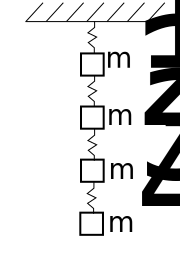
\includegraphics{../lecture_09/mass_springs.svg}
\caption{Springs-masses}
\end{figure}

The masses have the following amounts, 1, 2, 3, and 4 kg for masses 1-4.
Using a FBD for each mass:

\(m_{1}g+k_{2}(x_{2}-x_{1})-k_{1}x_{1}=0\)

\(m_{2}g+k_{3}(x_{3}-x_{2})-k_{2}(x_{2}-x_{1})=0\)

\(m_{3}g+k_{4}(x_{4}-x_{3})-k_{3}(x_{3}-x_{2})=0\)

\(m_{4}g-k_{4}(x_{4}-x_{3})=0\)

in matrix form:

\(\left[ \begin{array}{cccc} k_1+k_2 & -k_2 & 0 & 0 \\ -k_2 & k_2+k_3 & -k_3 & 0 \\ 0 & -k_3 & k_3+k_4 & -k_4 \\ 0 & 0 & -k_4 & k_4 \end{array} \right] \left[ \begin{array}{c} x_{1} \\ x_{2} \\ x_{3} \\ x_{4} \end{array} \right]= \left[ \begin{array}{c} m_{1}g \\ m_{2}g \\ m_{3}g \\ m_{4}g \end{array} \right]\)

    \begin{Verbatim}[commandchars=\\\{\}]
{\color{incolor}In [{\color{incolor}29}]:} \PY{n}{k1}\PY{p}{=}\PY{l+m+mi}{10}\PY{p}{;} \PY{n}{k2}\PY{p}{=}\PY{l+m+mi}{5}\PY{p}{;}\PY{n}{k3}\PY{p}{=}\PY{l+m+mi}{2}\PY{p}{;}\PY{n}{k4}\PY{p}{=}\PY{l+m+mi}{1}\PY{p}{;} \PY{c}{\PYZpc{} N/m}
         \PY{n}{m1}\PY{p}{=}\PY{l+m+mi}{1}\PY{p}{;} \PY{c}{\PYZpc{} kg}
         \PY{n}{m2}\PY{p}{=}\PY{l+m+mi}{2}\PY{p}{;}
         \PY{n}{m3}\PY{p}{=}\PY{l+m+mi}{3}\PY{p}{;}
         \PY{n}{m4}\PY{p}{=}\PY{l+m+mi}{4}\PY{p}{;}
         \PY{n}{g}\PY{p}{=}\PY{l+m+mf}{9.81}\PY{p}{;} \PY{c}{\PYZpc{} m/s\PYZca{}2}
         \PY{n}{K}\PY{p}{=}\PY{p}{[}\PY{n}{k1}\PY{o}{+}\PY{n}{k2} \PY{o}{\PYZhy{}}\PY{n}{k2} \PY{l+m+mi}{0} \PY{l+m+mi}{0}\PY{p}{;} \PY{o}{\PYZhy{}}\PY{n}{k2}\PY{p}{,} \PY{n}{k2}\PY{o}{+}\PY{n}{k3}\PY{p}{,} \PY{o}{\PYZhy{}}\PY{n}{k3} \PY{l+m+mi}{0}\PY{p}{;} \PY{l+m+mi}{0} \PY{o}{\PYZhy{}}\PY{n}{k3}\PY{p}{,} \PY{n}{k3}\PY{o}{+}\PY{n}{k4}\PY{p}{,} \PY{o}{\PYZhy{}}\PY{n}{k4}\PY{p}{;} \PY{l+m+mi}{0} \PY{l+m+mi}{0} \PY{o}{\PYZhy{}}\PY{n}{k4} \PY{n}{k4}\PY{p}{]}
         \PY{n}{y}\PY{p}{=}\PY{p}{[}\PY{n}{m1}\PY{o}{*}\PY{n}{g}\PY{p}{;}\PY{n}{m2}\PY{o}{*}\PY{n}{g}\PY{p}{;}\PY{n}{m3}\PY{o}{*}\PY{n}{g}\PY{p}{;}\PY{n}{m4}\PY{o}{*}\PY{n}{g}\PY{p}{]}
\end{Verbatim}

    \begin{Verbatim}[commandchars=\\\{\}]
K =

   15   -5    0    0
   -5    7   -2    0
    0   -2    3   -1
    0    0   -1    1

y =

    9.8100
   19.6200
   29.4300
   39.2400


    \end{Verbatim}

    \subsection{Tridiagonal matrix}\label{tridiagonal-matrix}

This matrix, K, could be rewritten as 3 vectors e, f and g

\(e=\left[ \begin{array}{c} 0 \\ -5 \\ -2 \\ -1 \end{array} \right]\)

\(f=\left[ \begin{array}{c} 15 \\ 7 \\ 3 \\ 1 \end{array} \right]\)

\(g=\left[ \begin{array}{c} -5 \\ -2 \\ -1 \\ 0 \end{array} \right]\)

Where all other components are 0 and the length of the vectors are n and
the first component of e and the last component of g are zero

\texttt{e(1)=0}

\texttt{g(end)=0}

No need to pivot and number of calculations reduced enormously.

\begin{longtable}[c]{@{}ll@{}}
\toprule
method & Number of Floating point operations for
n\(\times\)n-matrix\tabularnewline
\midrule
\endhead
Naive Gauss & n-cubed\tabularnewline
Tridiagonal & n\tabularnewline
\bottomrule
\end{longtable}

    \begin{Verbatim}[commandchars=\\\{\}]
{\color{incolor}In [{\color{incolor}30}]:} \PY{n+nb}{e}\PY{p}{=}\PY{p}{[}\PY{l+m+mi}{0}\PY{p}{;}\PY{o}{\PYZhy{}}\PY{l+m+mi}{5}\PY{p}{;}\PY{o}{\PYZhy{}}\PY{l+m+mi}{2}\PY{p}{;}\PY{o}{\PYZhy{}}\PY{l+m+mi}{1}\PY{p}{]}\PY{p}{;}
         \PY{n}{g}\PY{p}{=}\PY{p}{[}\PY{o}{\PYZhy{}}\PY{l+m+mi}{5}\PY{p}{;}\PY{o}{\PYZhy{}}\PY{l+m+mi}{2}\PY{p}{;}\PY{o}{\PYZhy{}}\PY{l+m+mi}{1}\PY{p}{;}\PY{l+m+mi}{0}\PY{p}{]}\PY{p}{;}
         \PY{n}{f}\PY{p}{=}\PY{p}{[}\PY{l+m+mi}{15}\PY{p}{;}\PY{l+m+mi}{7}\PY{p}{;}\PY{l+m+mi}{3}\PY{p}{;}\PY{l+m+mi}{1}\PY{p}{]}\PY{p}{;}
         \PY{n}{Tridiag}\PY{p}{(}\PY{n+nb}{e}\PY{p}{,}\PY{n}{f}\PY{p}{,}\PY{n}{g}\PY{p}{,}\PY{n}{y}\PY{p}{)}
\end{Verbatim}

    \begin{Verbatim}[commandchars=\\\{\}]
ans =

     9.8100    27.4680    61.8030   101.0430


    \end{Verbatim}

    \begin{Verbatim}[commandchars=\\\{\}]
{\color{incolor}In [{\color{incolor}12}]:} \PY{c}{\PYZpc{} tic ... t=toc }
         \PY{c}{\PYZpc{} is Matlab timer used for debugging programs}
         \PY{n}{t\PYZus{}GE} \PY{p}{=} \PY{n+nb}{zeros}\PY{p}{(}\PY{l+m+mi}{1}\PY{p}{,}\PY{l+m+mi}{100}\PY{p}{)}\PY{p}{;}
         \PY{n}{t\PYZus{}GE\PYZus{}tridiag} \PY{p}{=} \PY{n+nb}{zeros}\PY{p}{(}\PY{l+m+mi}{1}\PY{p}{,}\PY{l+m+mi}{100}\PY{p}{)}\PY{p}{;}
         \PY{n}{t\PYZus{}TD} \PY{p}{=} \PY{n+nb}{zeros}\PY{p}{(}\PY{l+m+mi}{1}\PY{p}{,}\PY{l+m+mi}{100}\PY{p}{)}\PY{p}{;}
         \PY{c}{\PYZpc{}for n = 1:200}
         \PY{k}{for} \PY{n}{n}\PY{p}{=}\PY{l+m+mi}{1}\PY{p}{:}\PY{l+m+mi}{100}
             \PY{n}{A} \PY{p}{=} \PY{n+nb}{rand}\PY{p}{(}\PY{n}{n}\PY{p}{,}\PY{n}{n}\PY{p}{)}\PY{p}{;}
             \PY{n+nb}{e} \PY{p}{=} \PY{n+nb}{rand}\PY{p}{(}\PY{n}{n}\PY{p}{,}\PY{l+m+mi}{1}\PY{p}{)}\PY{p}{;} \PY{n+nb}{e}\PY{p}{(}\PY{l+m+mi}{1}\PY{p}{)}\PY{p}{=}\PY{l+m+mi}{0}\PY{p}{;}
             \PY{n}{f} \PY{p}{=} \PY{n+nb}{rand}\PY{p}{(}\PY{n}{n}\PY{p}{,}\PY{l+m+mi}{1}\PY{p}{)}\PY{p}{;}
             \PY{n}{g} \PY{p}{=} \PY{n+nb}{rand}\PY{p}{(}\PY{n}{n}\PY{p}{,}\PY{l+m+mi}{1}\PY{p}{)}\PY{p}{;} \PY{n}{g}\PY{p}{(}\PY{k}{end}\PY{p}{)}\PY{p}{=}\PY{l+m+mi}{0}\PY{p}{;}
             \PY{n}{Atd}\PY{p}{=}\PY{n+nb}{diag}\PY{p}{(}\PY{n}{f}\PY{p}{,} \PY{l+m+mi}{0}\PY{p}{)} \PY{o}{\PYZhy{}} \PY{n+nb}{diag}\PY{p}{(}\PY{n+nb}{e}\PY{p}{(}\PY{l+m+mi}{2}\PY{p}{:}\PY{n}{n}\PY{p}{)}\PY{p}{,} \PY{o}{\PYZhy{}}\PY{l+m+mi}{1}\PY{p}{)} \PY{o}{\PYZhy{}} \PY{n+nb}{diag}\PY{p}{(}\PY{n}{g}\PY{p}{(}\PY{l+m+mi}{1}\PY{p}{:}\PY{n}{n}\PY{o}{\PYZhy{}}\PY{l+m+mi}{1}\PY{p}{)}\PY{p}{,} \PY{l+m+mi}{1}\PY{p}{)}\PY{p}{;}
             \PY{n}{b} \PY{p}{=} \PY{n+nb}{rand}\PY{p}{(}\PY{n}{n}\PY{p}{,}\PY{l+m+mi}{1}\PY{p}{)}\PY{p}{;}
             \PY{n+nb}{tic}\PY{p}{;}
             \PY{n}{x} \PY{p}{=} \PY{n}{GaussPivot}\PY{p}{(}\PY{n}{A}\PY{p}{,}\PY{n}{b}\PY{p}{)}\PY{p}{;}
             \PY{n}{t\PYZus{}GE}\PY{p}{(}\PY{n}{n}\PY{p}{)} \PY{p}{=} \PY{n+nb}{toc}\PY{p}{;}
             \PY{n+nb}{tic}\PY{p}{;}
             \PY{n}{x} \PY{p}{=} \PY{n}{GaussPivot}\PY{p}{(}\PY{n}{Atd}\PY{p}{,}\PY{n}{b}\PY{p}{)}\PY{p}{;}
             \PY{n}{t\PYZus{}GE\PYZus{}tridiag}\PY{p}{(}\PY{n}{n}\PY{p}{)} \PY{p}{=} \PY{n+nb}{toc}\PY{p}{;}
             \PY{n+nb}{tic}\PY{p}{;}
             \PY{n}{x} \PY{p}{=} \PY{n}{Tridiag}\PY{p}{(}\PY{n+nb}{e}\PY{p}{,}\PY{n}{f}\PY{p}{,}\PY{n}{g}\PY{p}{,}\PY{n}{b}\PY{p}{)}\PY{p}{;}
             \PY{n}{t\PYZus{}TD}\PY{p}{(}\PY{n}{n}\PY{p}{)} \PY{p}{=} \PY{n+nb}{toc}\PY{p}{;}
         \PY{k}{end}
\end{Verbatim}

    \begin{Verbatim}[commandchars=\\\{\}]
{\color{incolor}In [{\color{incolor}13}]:} \PY{n}{n}\PY{p}{=}\PY{l+m+mi}{1}\PY{p}{:}\PY{l+m+mi}{200}\PY{p}{;}
         \PY{n+nb}{loglog}\PY{p}{(}\PY{n}{n}\PY{p}{,}\PY{n}{t\PYZus{}GE}\PY{p}{,}\PY{n}{n}\PY{p}{,}\PY{n}{t\PYZus{}TD}\PY{p}{,}\PY{n}{n}\PY{p}{,}\PY{n}{t\PYZus{}GE\PYZus{}tridiag}\PY{p}{)}
         \PY{n+nb}{xlabel}\PY{p}{(}\PY{l+s}{\PYZsq{}}\PY{l+s}{number of elements\PYZsq{}}\PY{p}{)}
         \PY{n+nb}{ylabel}\PY{p}{(}\PY{l+s}{\PYZsq{}}\PY{l+s}{time (s)\PYZsq{}}\PY{p}{)}
\end{Verbatim}

    \begin{center}
    \adjustimage{max size={0.9\linewidth}{0.9\paperheight}}{lecture_10_files/lecture_10_27_0.pdf}
    \end{center}
    { \hspace*{\fill} \\}
    
    \begin{Verbatim}[commandchars=\\\{\}]
{\color{incolor}In [{\color{incolor} }]:} 
\end{Verbatim}


    % Add a bibliography block to the postdoc
    
    
    
    \end{document}
